% \begin{figure}%[!b]
% \begin{subfigure}{0.5\textwidth}
% 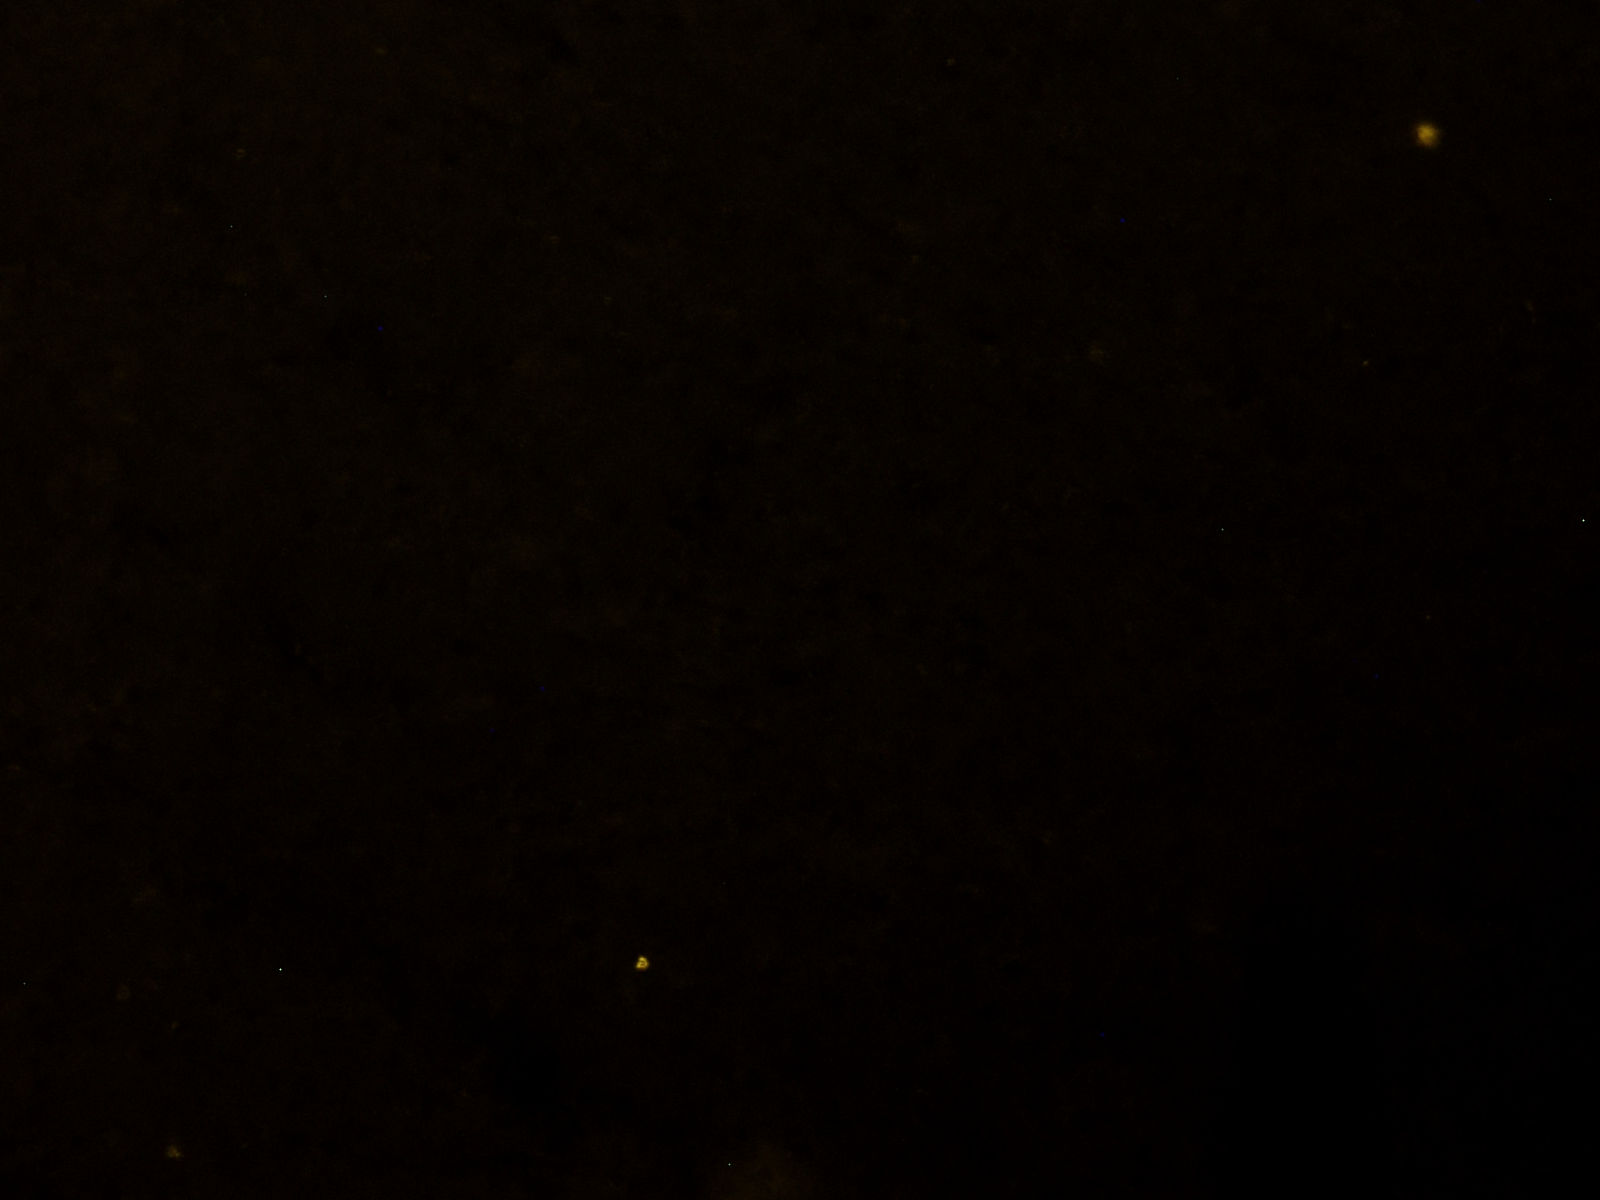
\includegraphics[width=\linewidth]{figures/120_dataset/i_empty.png}
% \subcaption{}
% \end{subfigure}%
% \begin{subfigure}{0.5\textwidth}
% 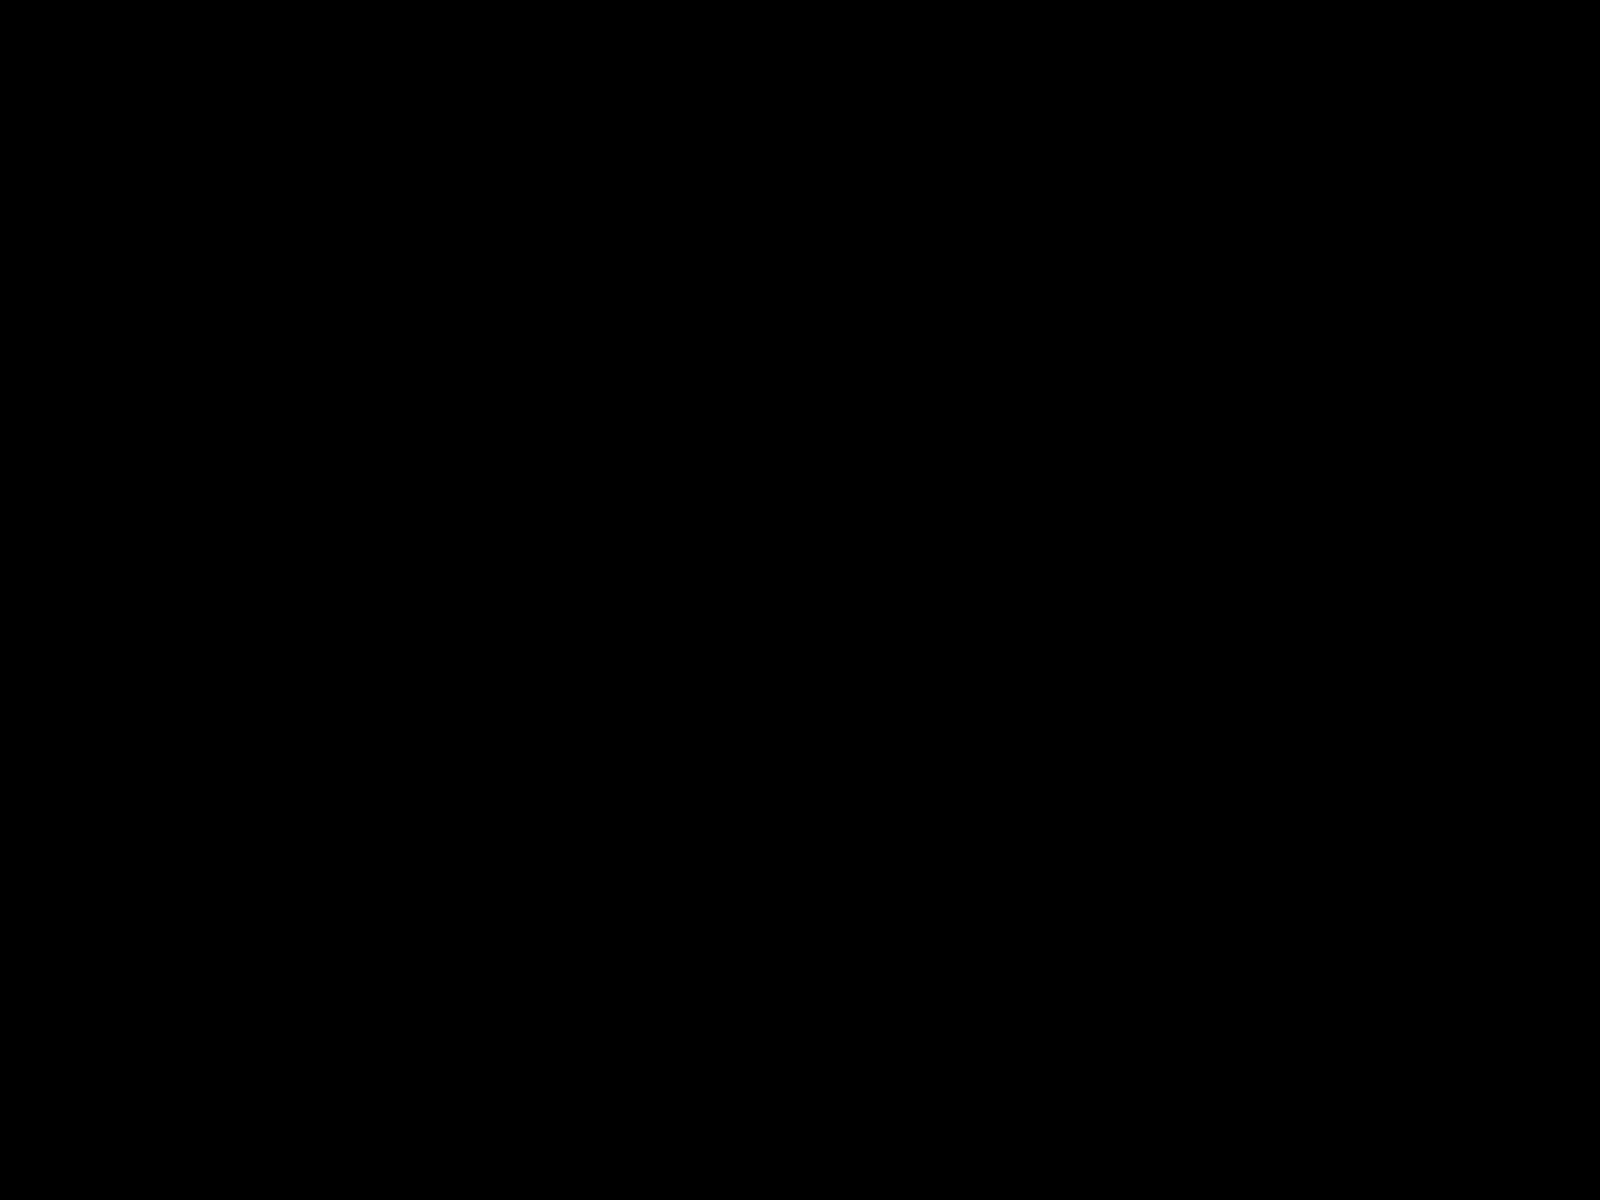
\includegraphics[width=\linewidth]{figures/120_dataset/m_empty.png}
% \subcaption{}
% \label{fig:dataset:empty}
% \end{subfigure}

% \centering
% \begin{subfigure}{0.5\textwidth}
% 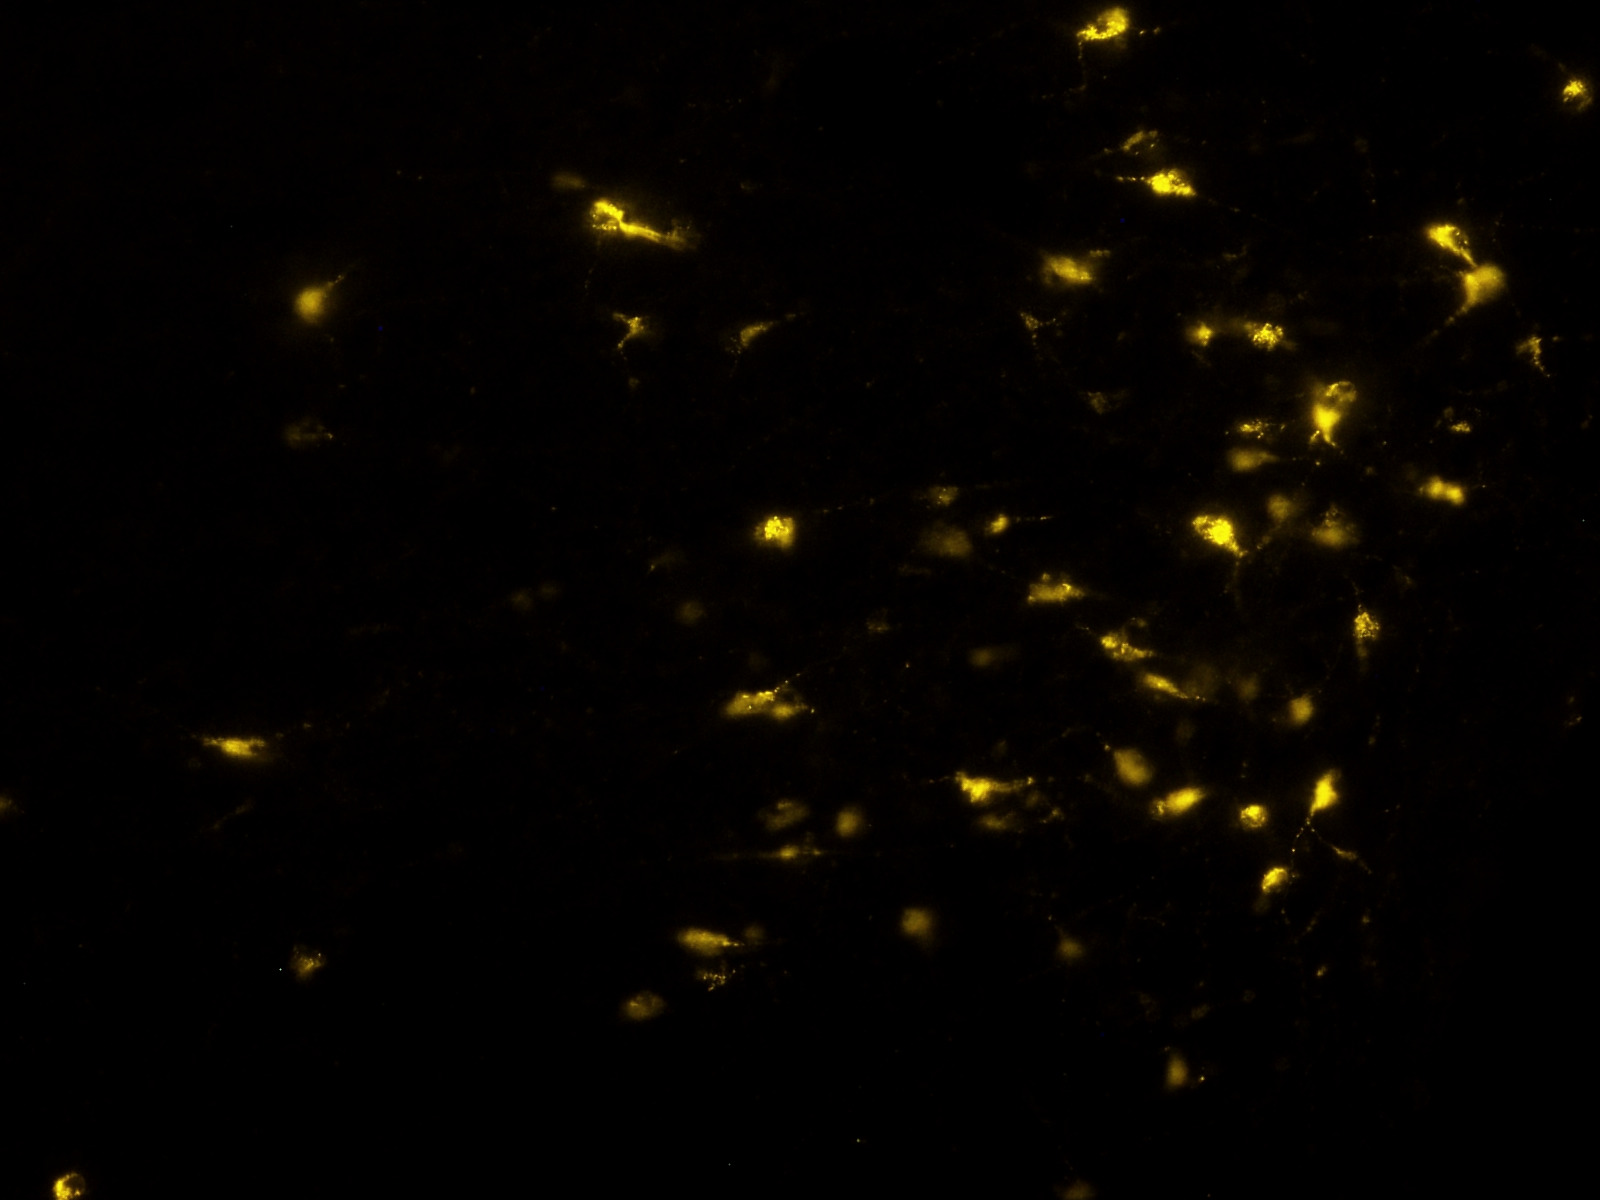
\includegraphics[width=\linewidth]{figures/120_dataset/i_168.jpeg}
% \subcaption{}
% \end{subfigure}%
% \begin{subfigure}{0.5\textwidth}
% 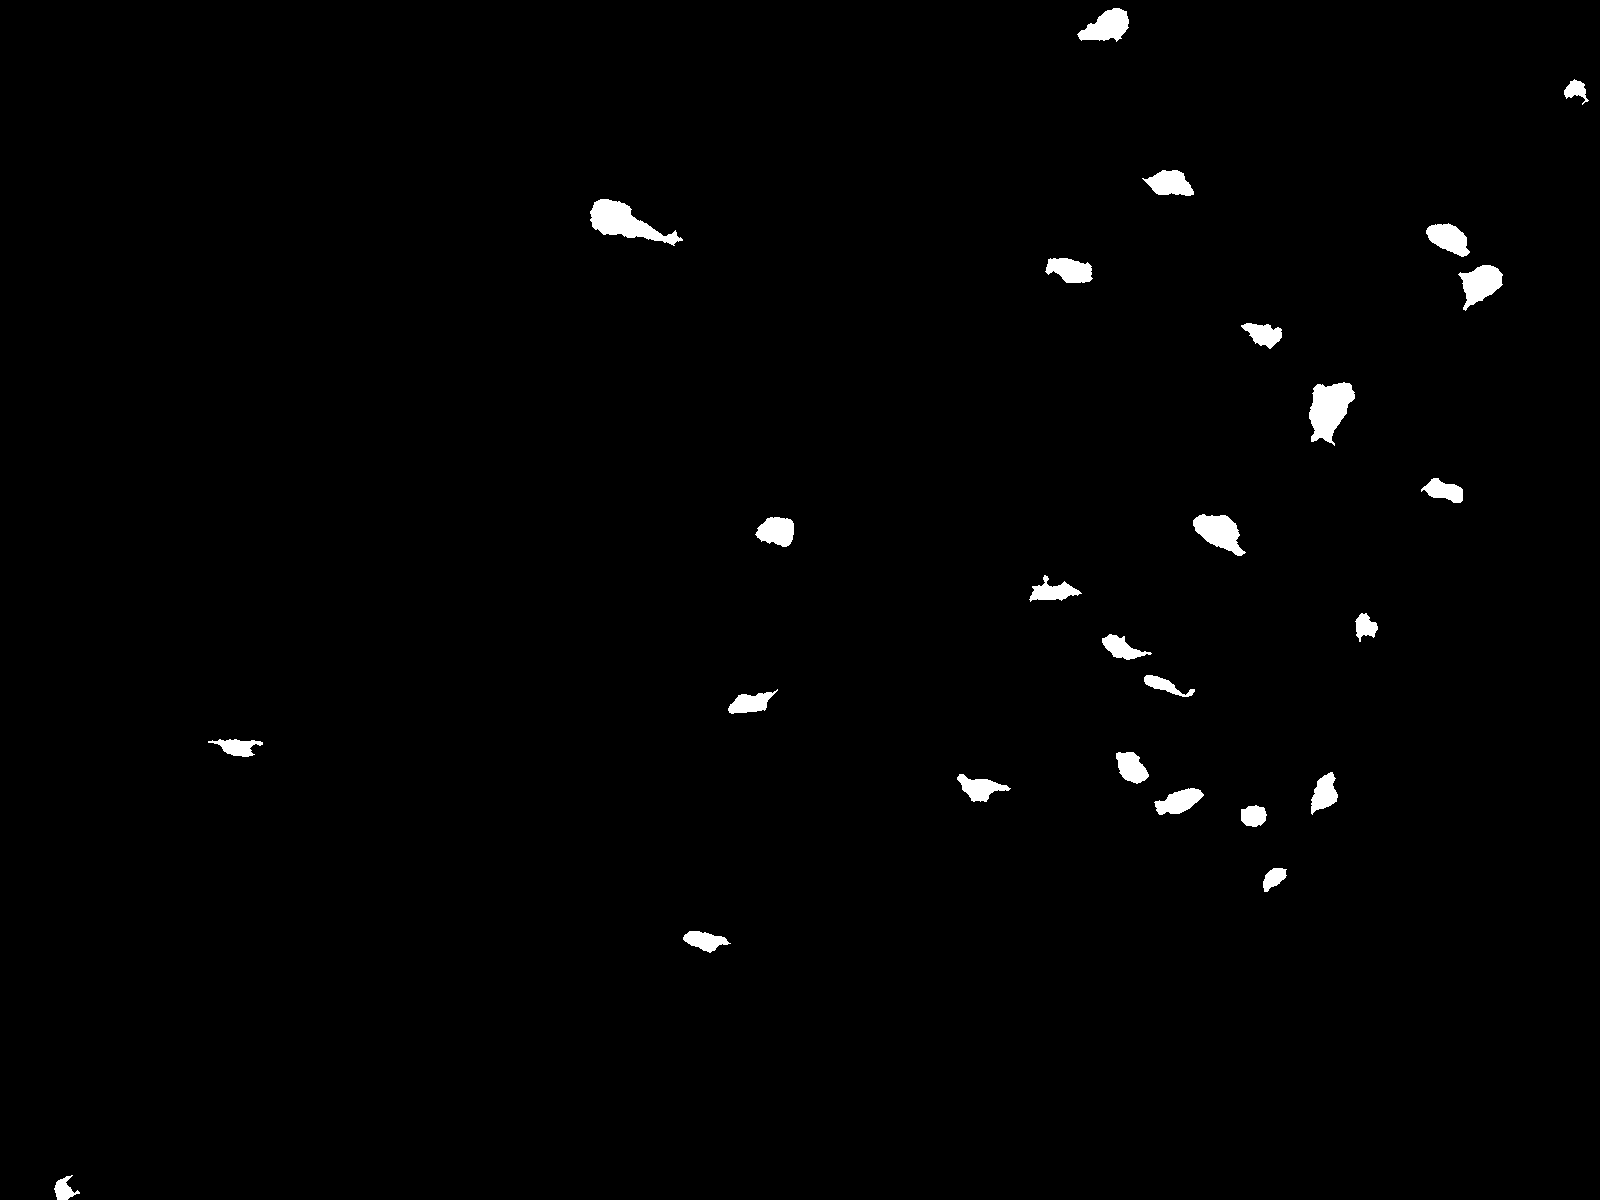
\includegraphics[width=\linewidth]{figures/120_dataset/m_168.png}
% \subcaption{}
% \label{fig:dataset:dark}
% \end{subfigure}

% \centering
% \begin{subfigure}{0.5\textwidth}
% 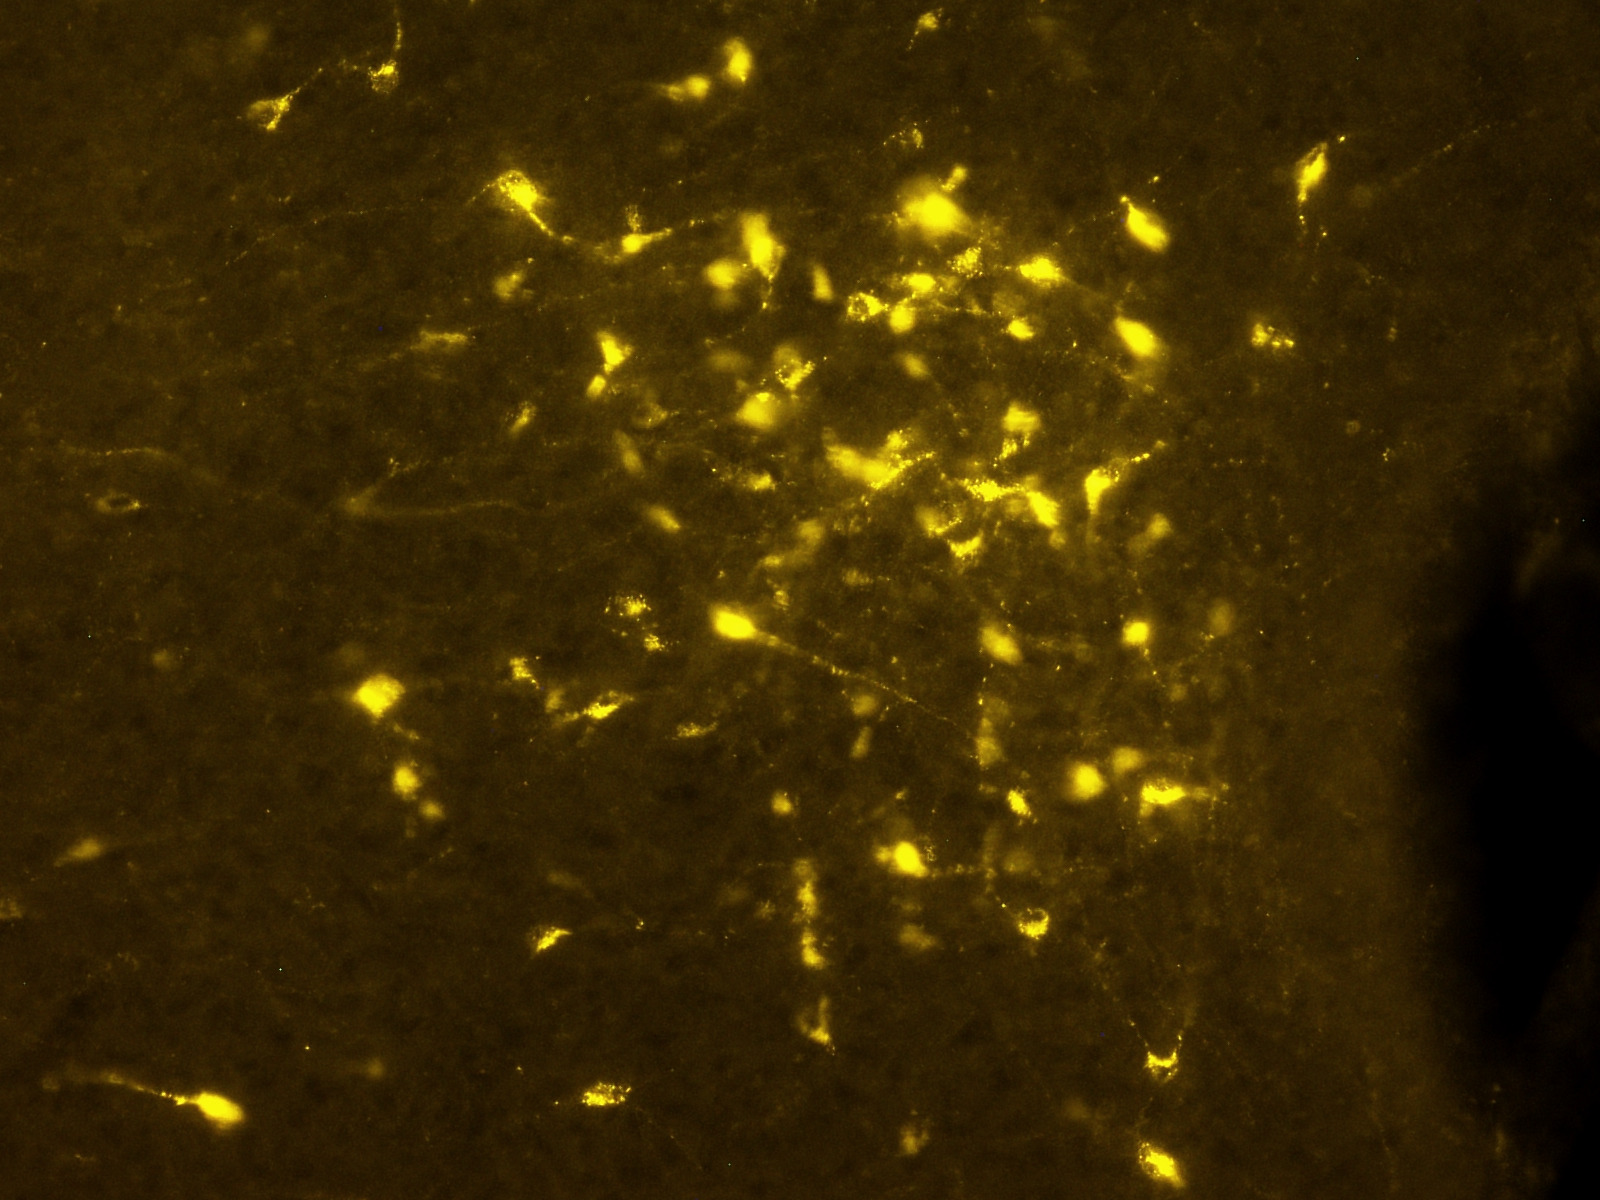
\includegraphics[width=\linewidth]{figures/120_dataset/i_257.jpeg}
% \subcaption{}
% \end{subfigure}%
% \begin{subfigure}{0.5\textwidth}
% 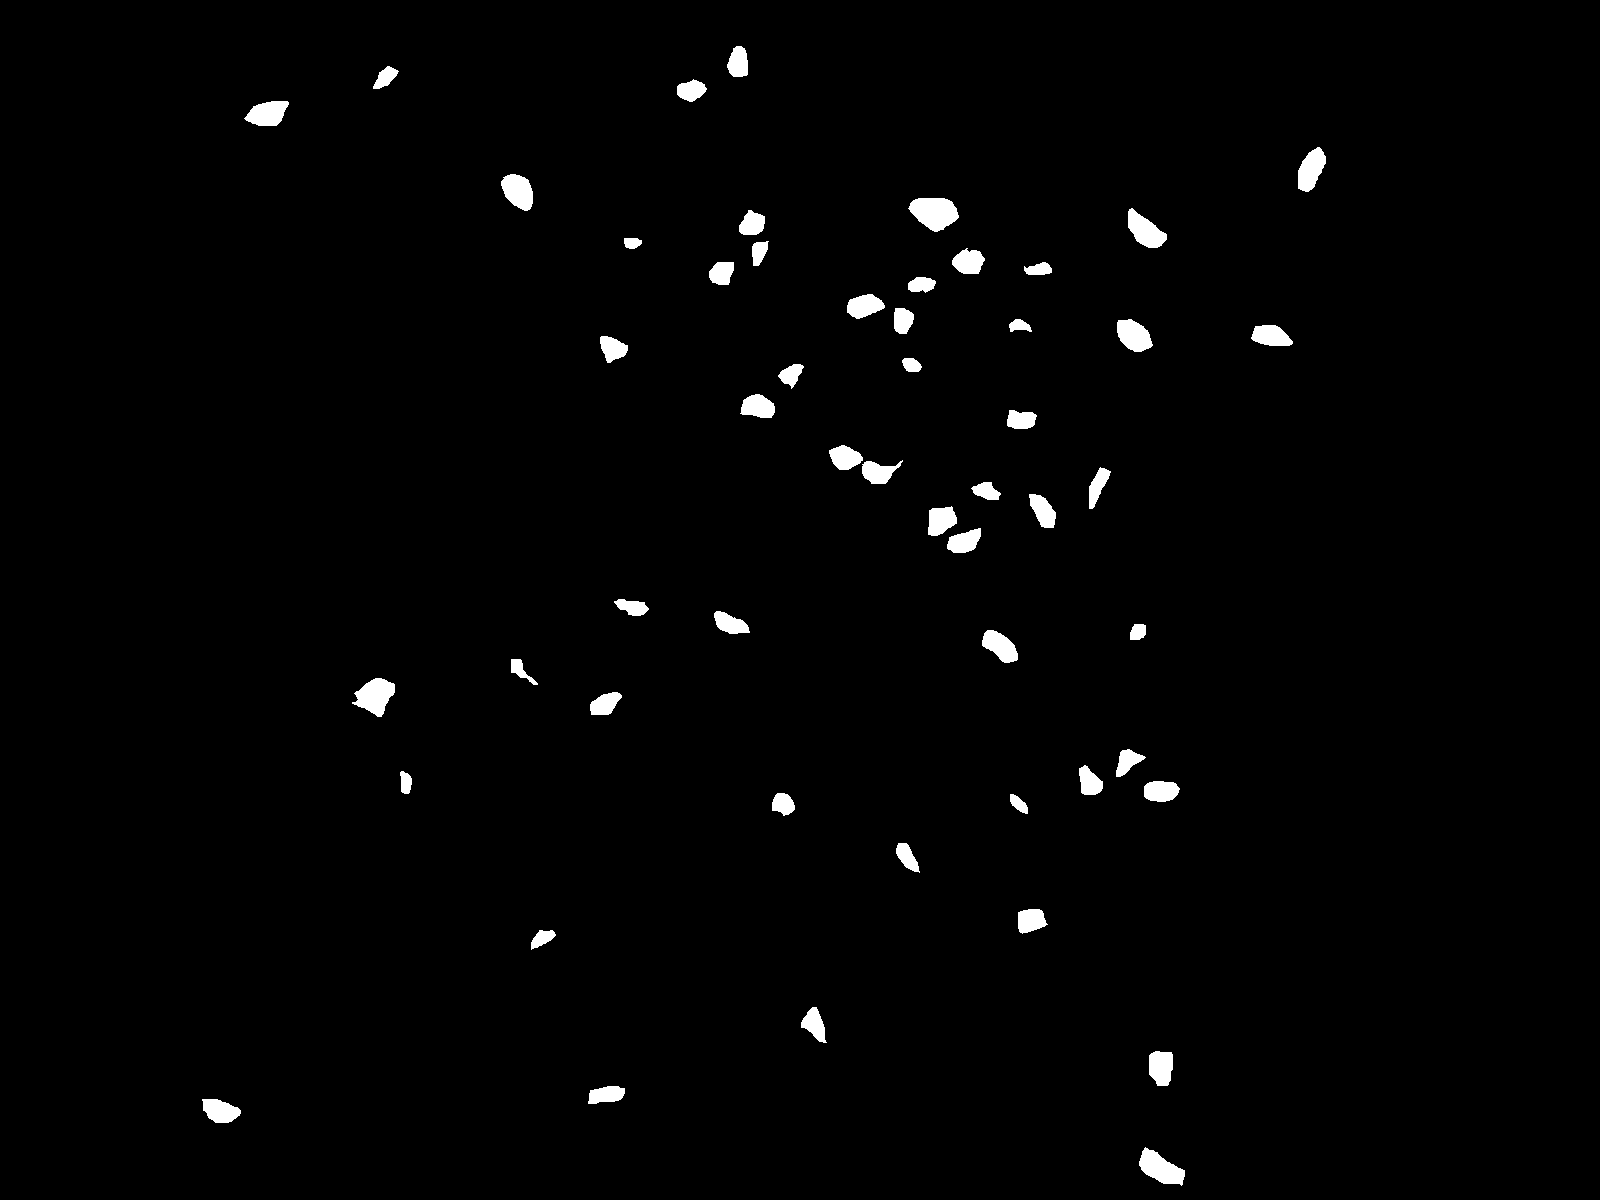
\includegraphics[width=\linewidth]{figures/120_dataset/m_257.png}
% \subcaption{}
% \label{fig:dataset:bright}
% \end{subfigure}
% \vspace{-0.2cm}
% \caption{
% \textbf{Sample data}. 
% Original images (left) and corresponding ground-truth masks (right).
% % The original images (left) present neuronal cells of different shape, size and saturation over a background of variable brightness and color.
% % The corresponding ground-truth masks used for training (right) depicts cells as white pixels over a black background.
% } \label{fig:dataset}
% \end{figure}%
% \begin{figure}%[ht]\ContinuedFloat
% \centering
% \begin{subfigure}{0.5\textwidth}
% 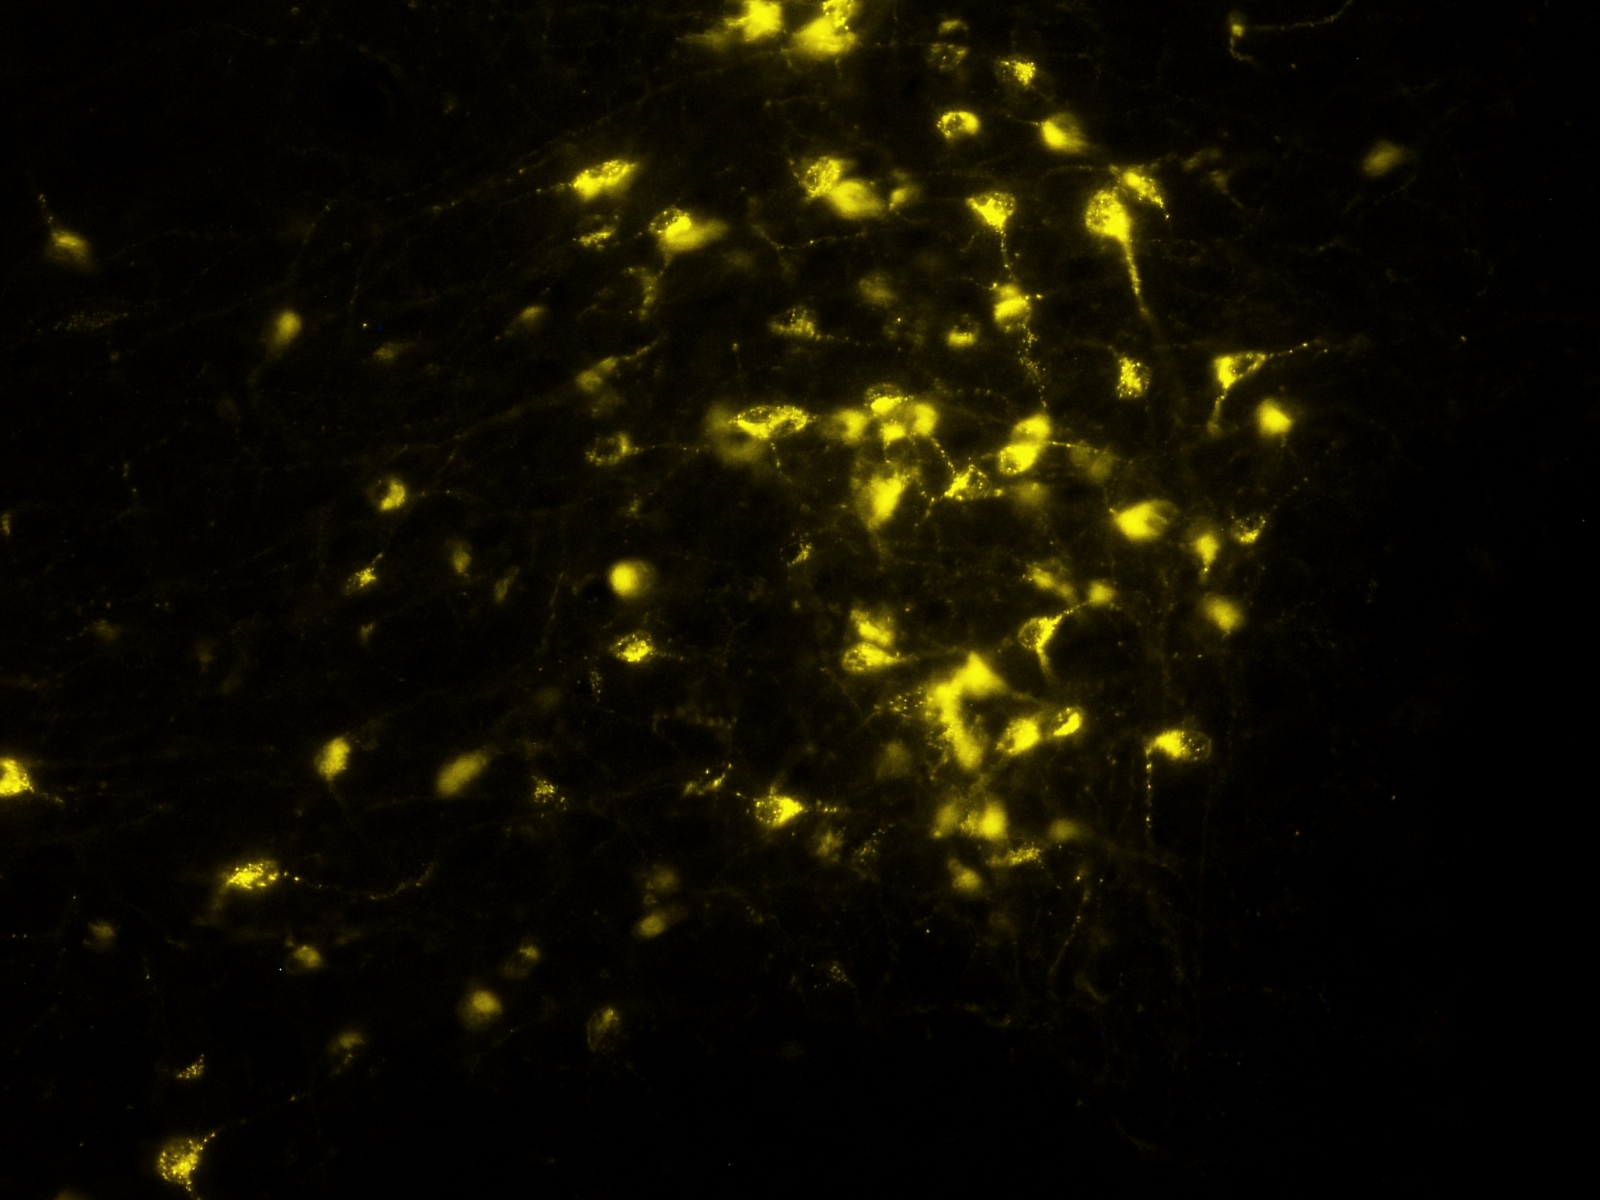
\includegraphics[width=\linewidth]{figures/120_dataset/i_clumping_yellow.png}
% \subcaption{}
% \end{subfigure}%
% \begin{subfigure}{0.5\textwidth}
% 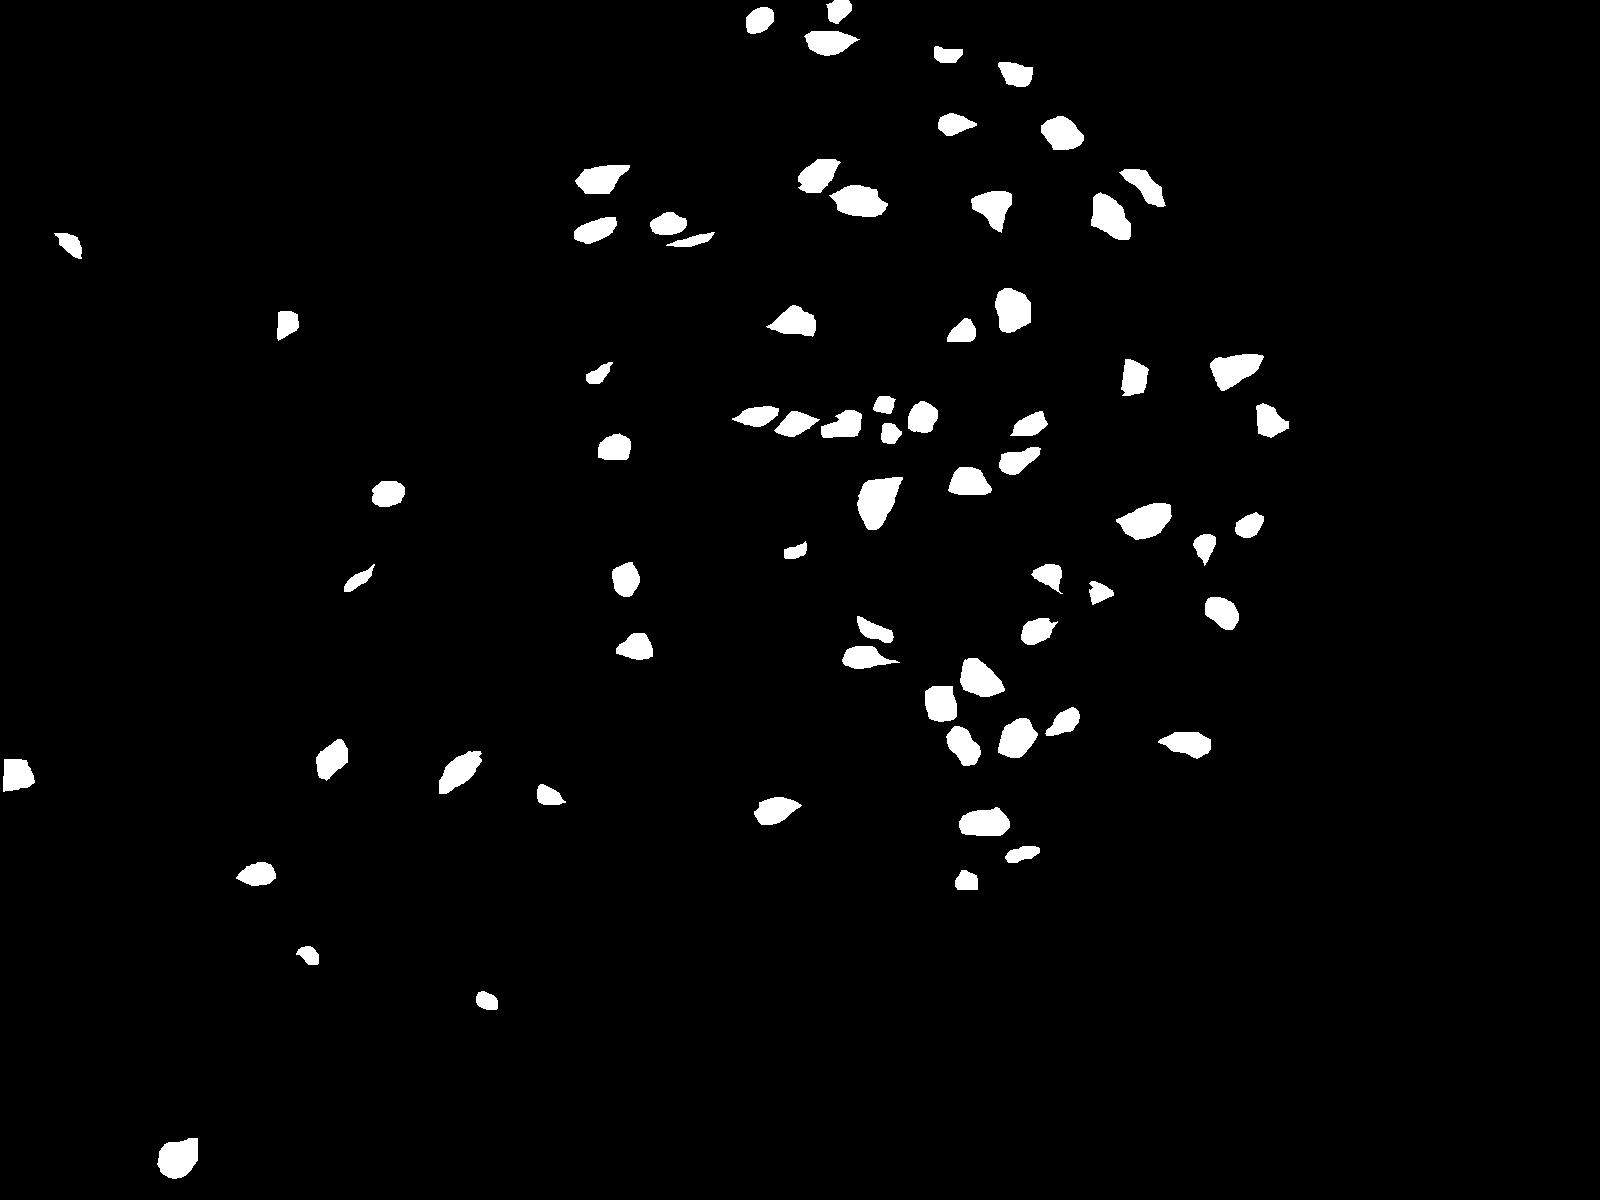
\includegraphics[width=\linewidth]{figures/120_dataset/m_clumping_yellow.png}
% \subcaption{}
% \label{fig:artifacts:clumping}
% \end{subfigure}

\savegeometry{origigeom}
\clearpage
\newgeometry{lmargin=1.5cm}
\begin{landscape}
\begin{figure}[!b]
    \centering
    \subfloat[Challenges]{
    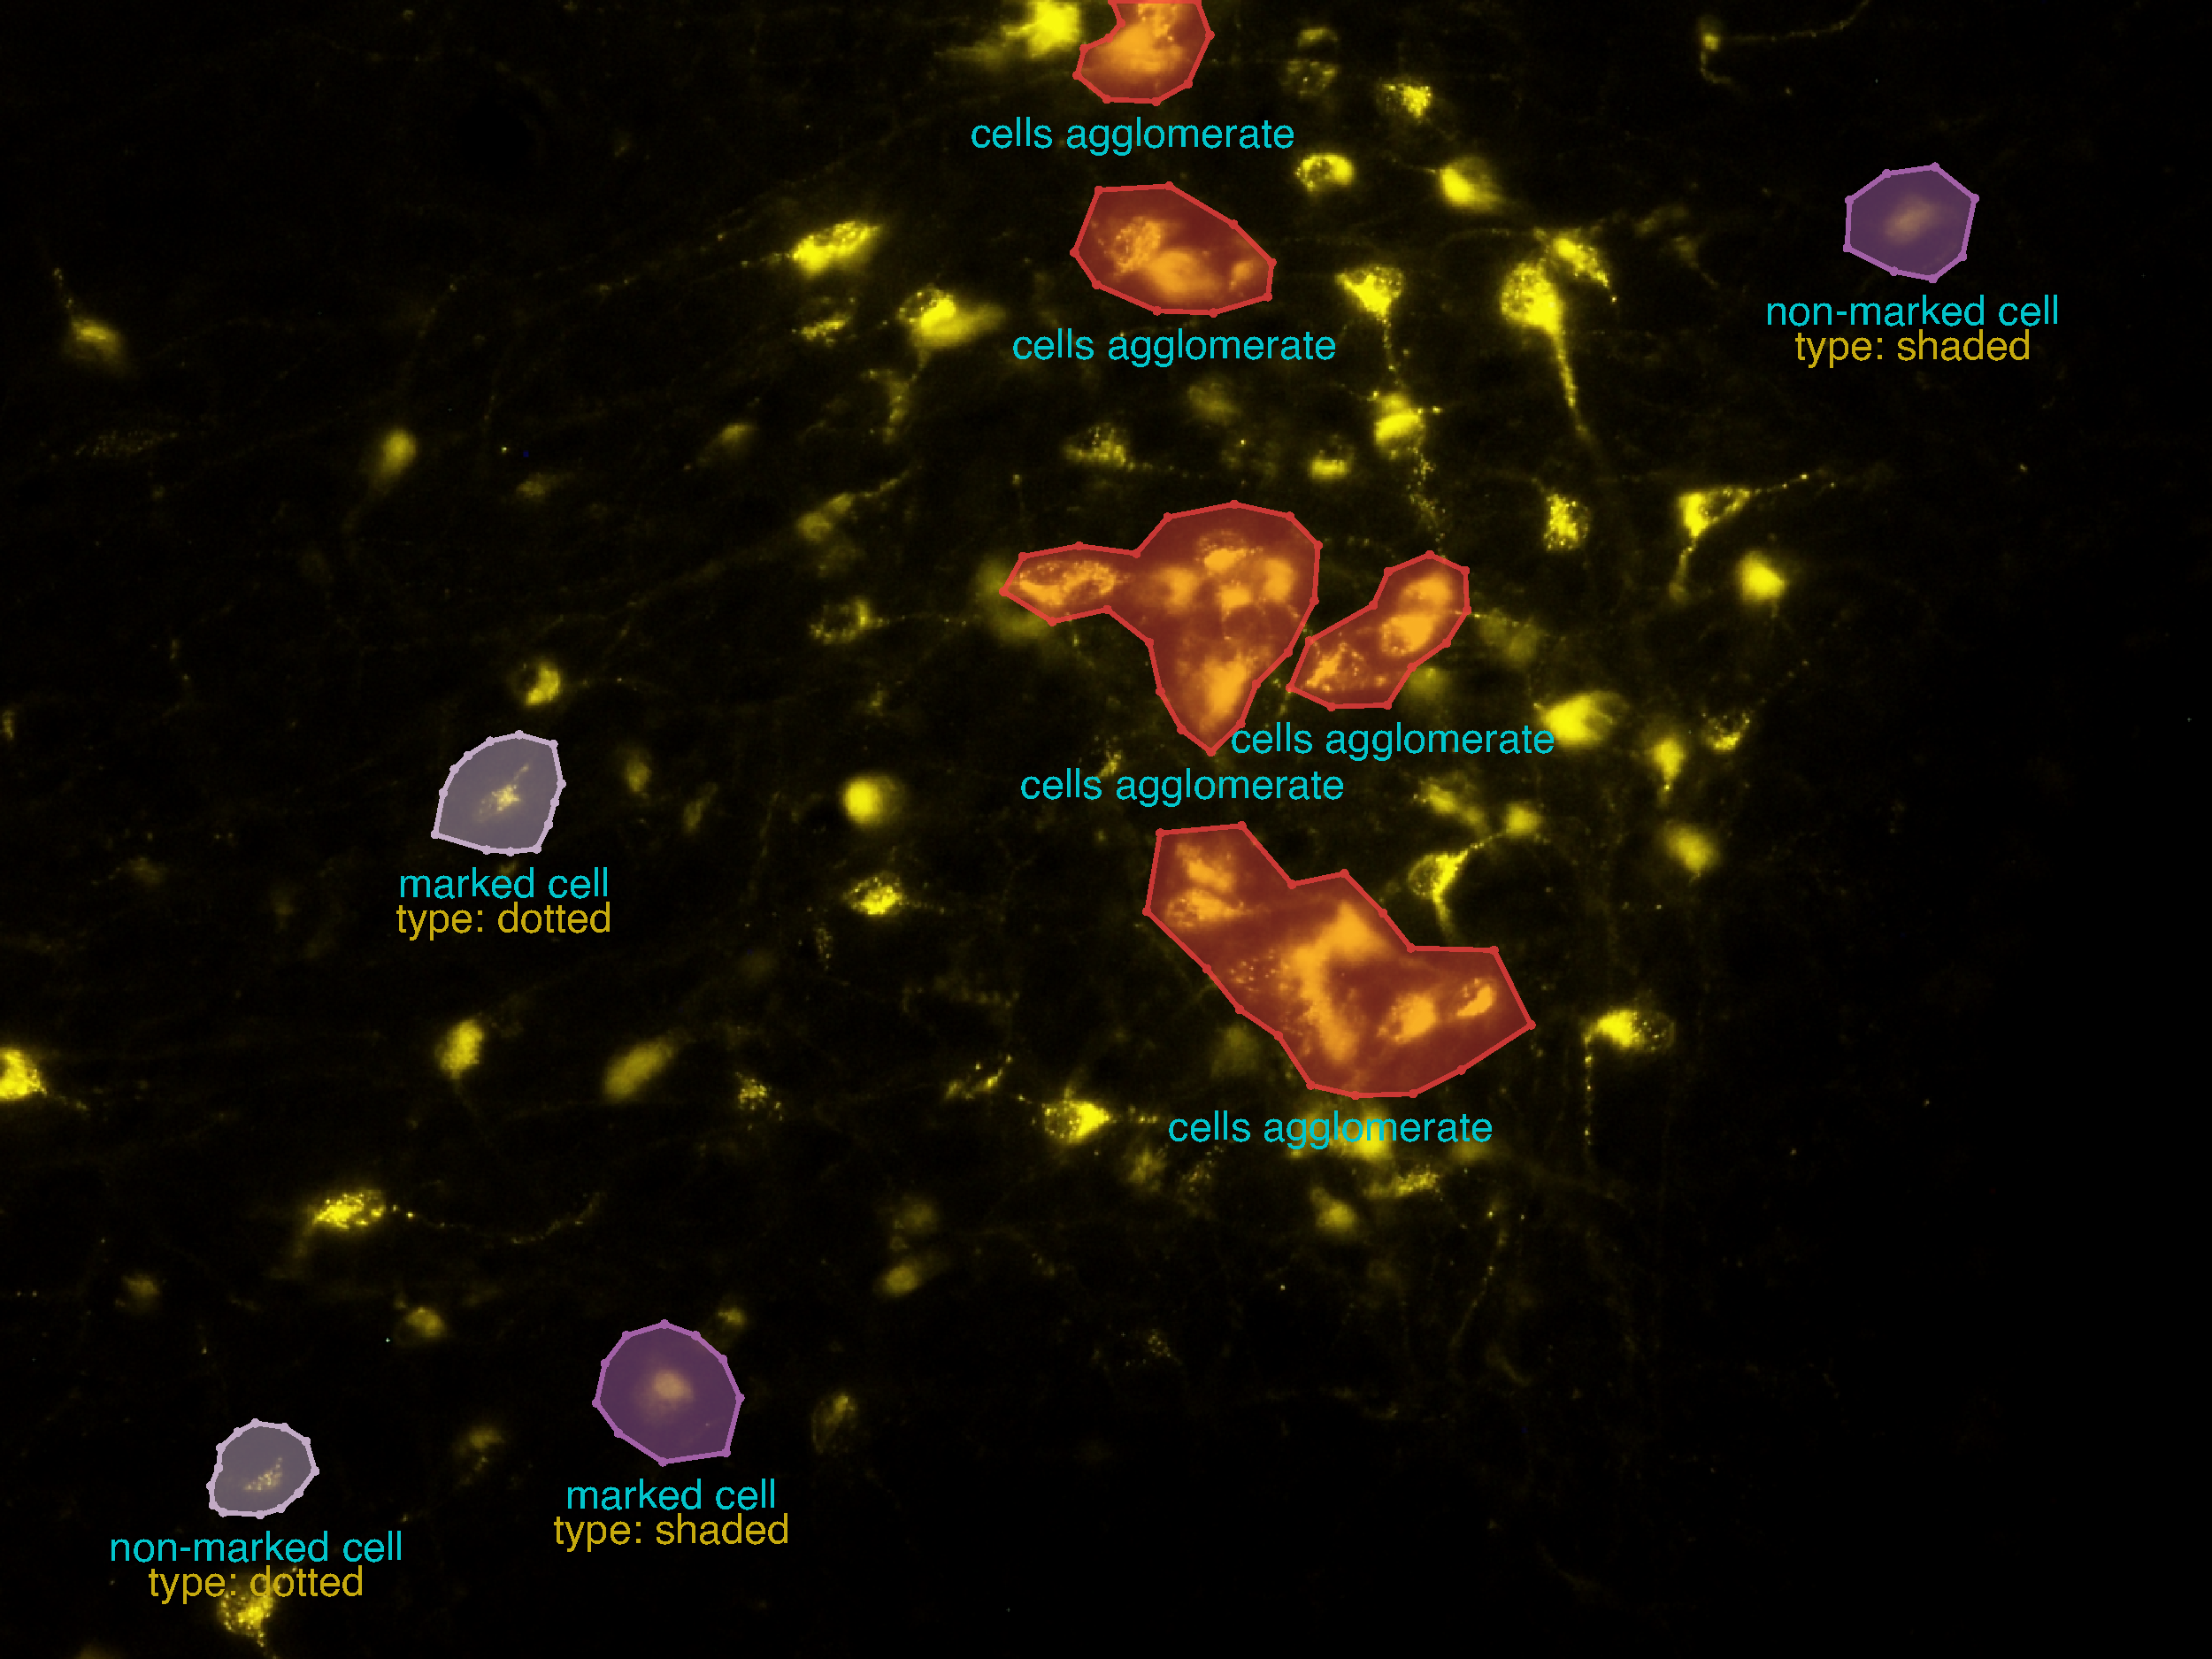
\includegraphics[width=\linewidth]{figures/120_dataset/challenges/challenges.pdf}\label{fig:artifacts:clumping}
    }
    \caption{\textbf{Challenges and artifacts.}
    Some of the images present cells agglomerate that require sharp boundary segmentation. 
    Also, marked cells may look very similar to non-marked objects due to an intrinsic arbitrariness of the recognition task.
    }
    \label{fig:artifacts}
\end{figure}%
% \end{landscape}

% \begin{landscape}
\begin{figure}[ht]\ContinuedFloat
    \centering
    \subfloat[Biological artifacts]{
    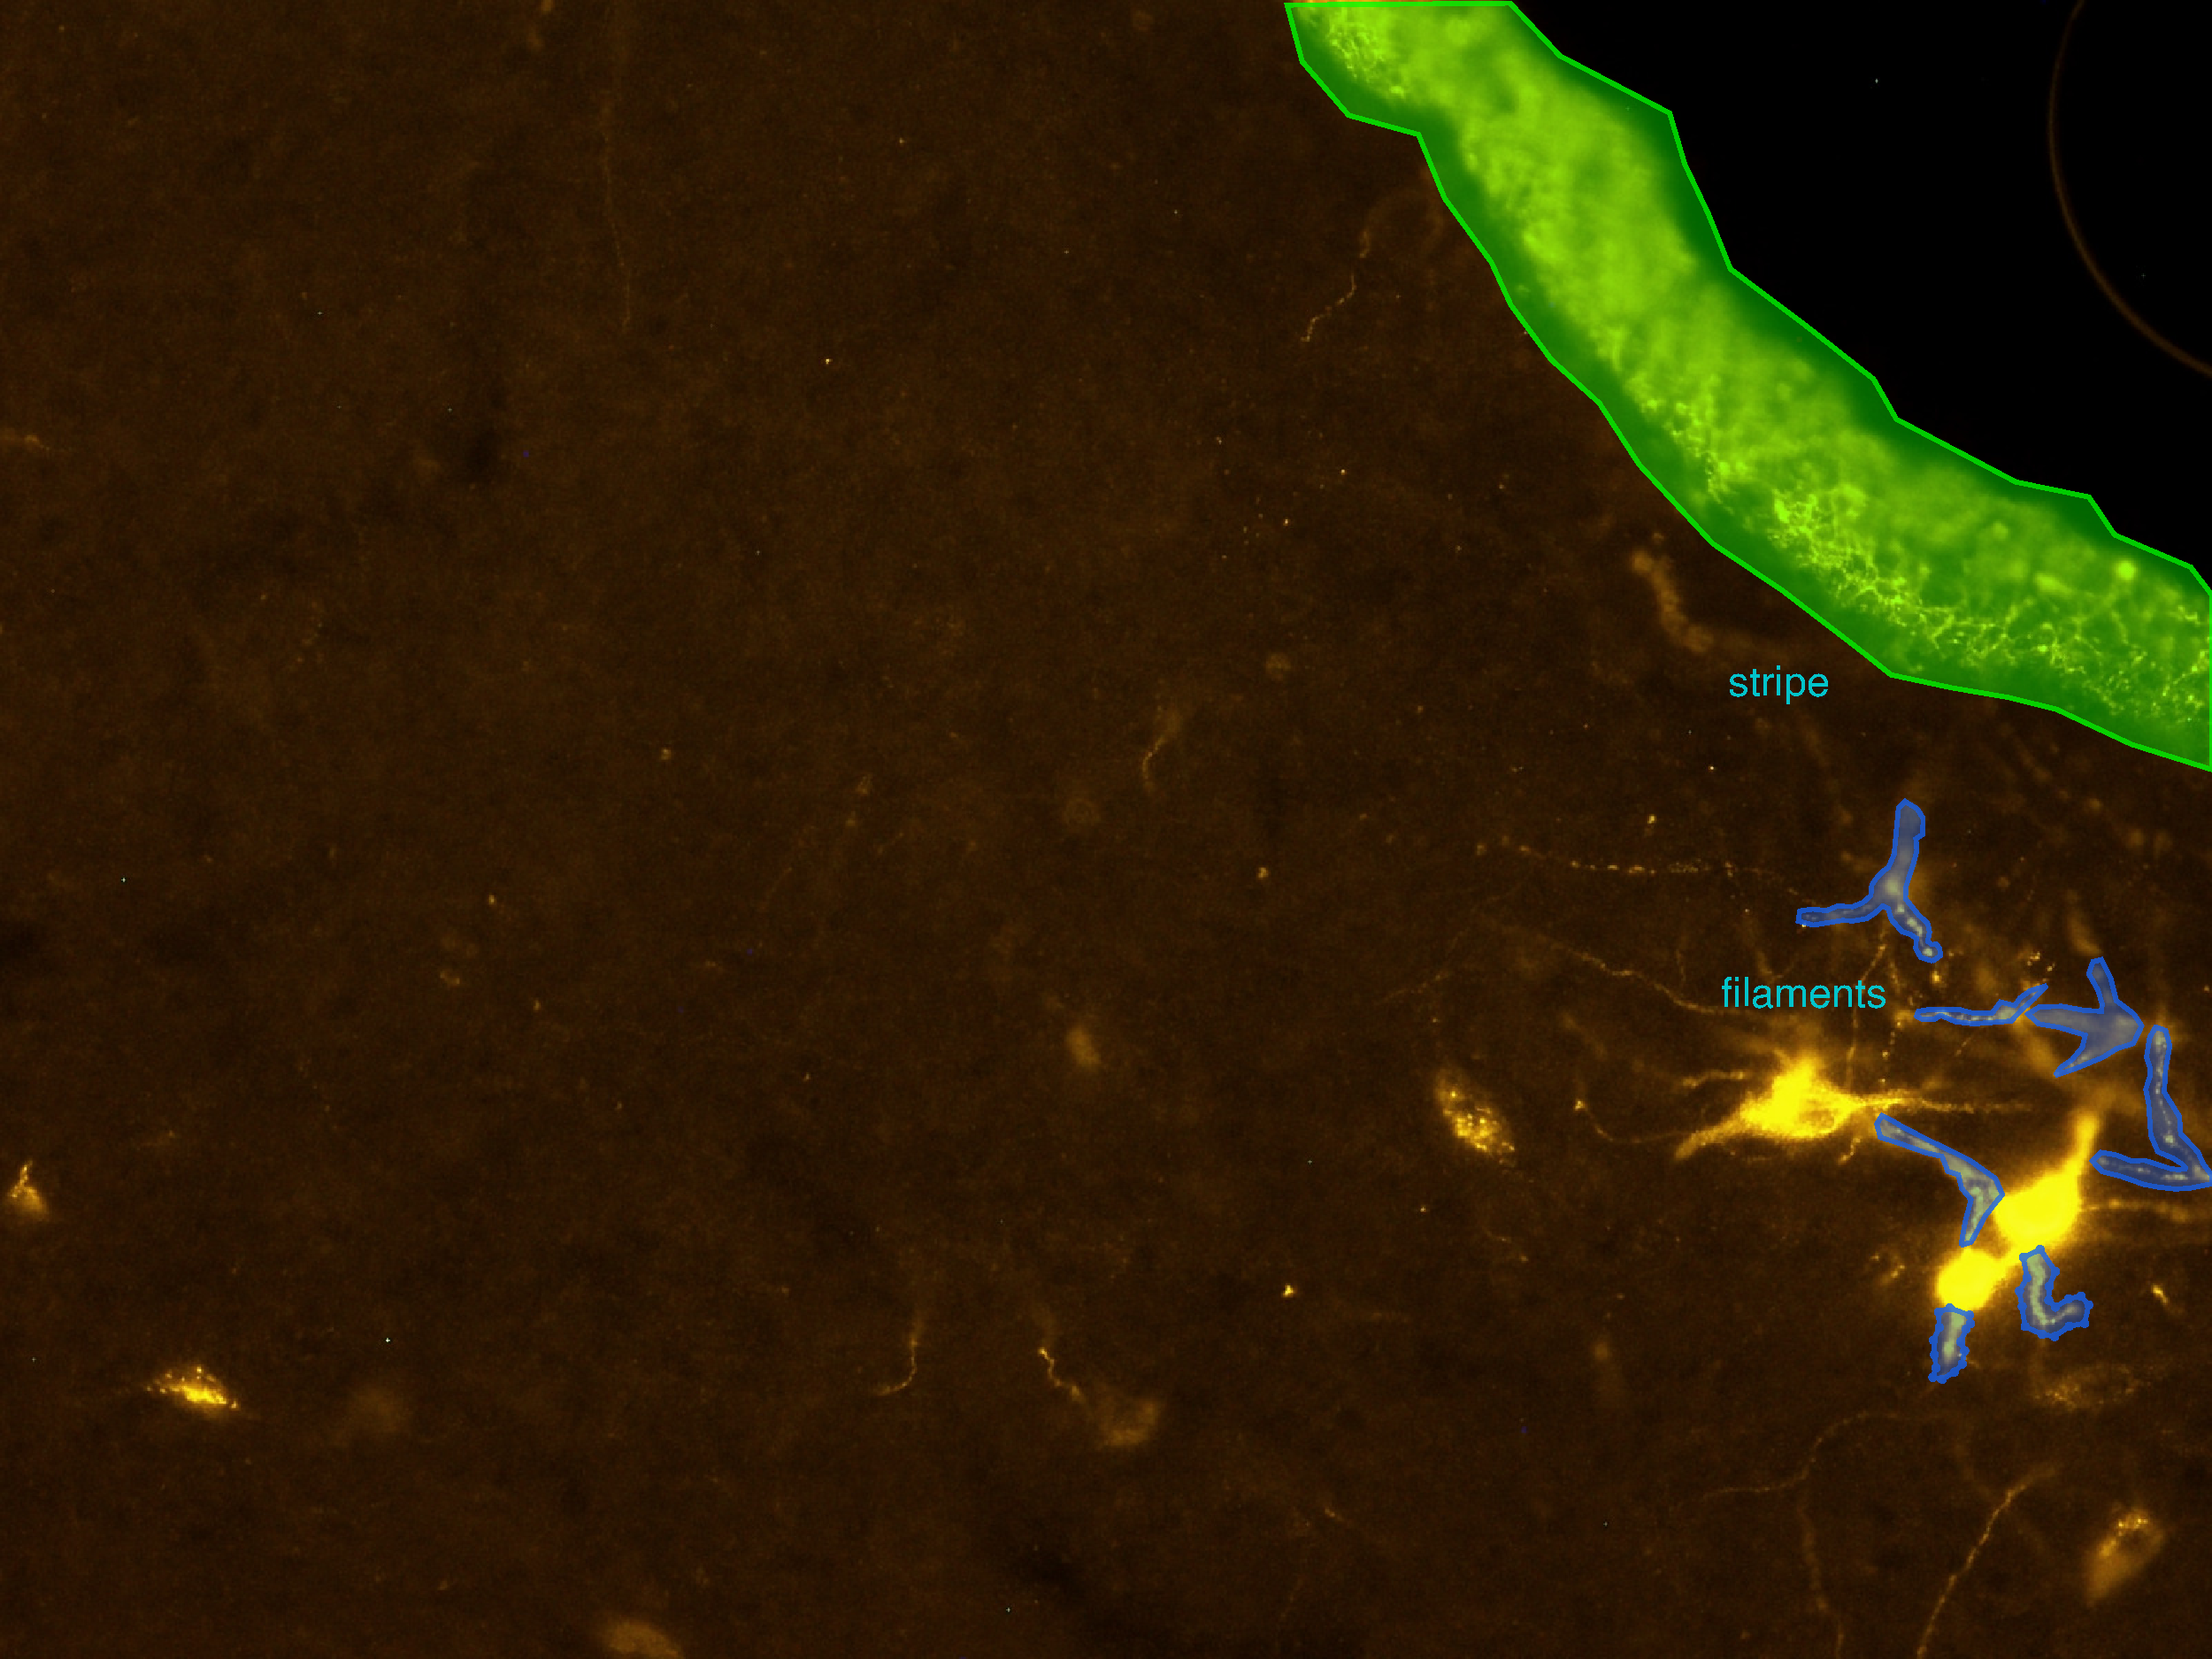
\includegraphics[width=\linewidth]{figures/120_dataset/challenges/stripe_and_filaments.pdf}\label{fig:artifacts:stripe}
    }
    \caption{\textbf{Challenges and artifacts. (2)}
    Although biological structures as the tissue border (stripe) or the axons (filaments) naturally have similar emission properties compared to neuronal cells, they are not of interest and ought to be discarded by the model.
    % some pictures present biological structures, as the stripe and the filaments in the figure, that are not of interest for our use case
    }
\end{figure}%
% \end{landscape}

% \begin{landscape}
\begin{figure}[ht]\ContinuedFloat
    \centering
    \subfloat[Technical artifacts]{
    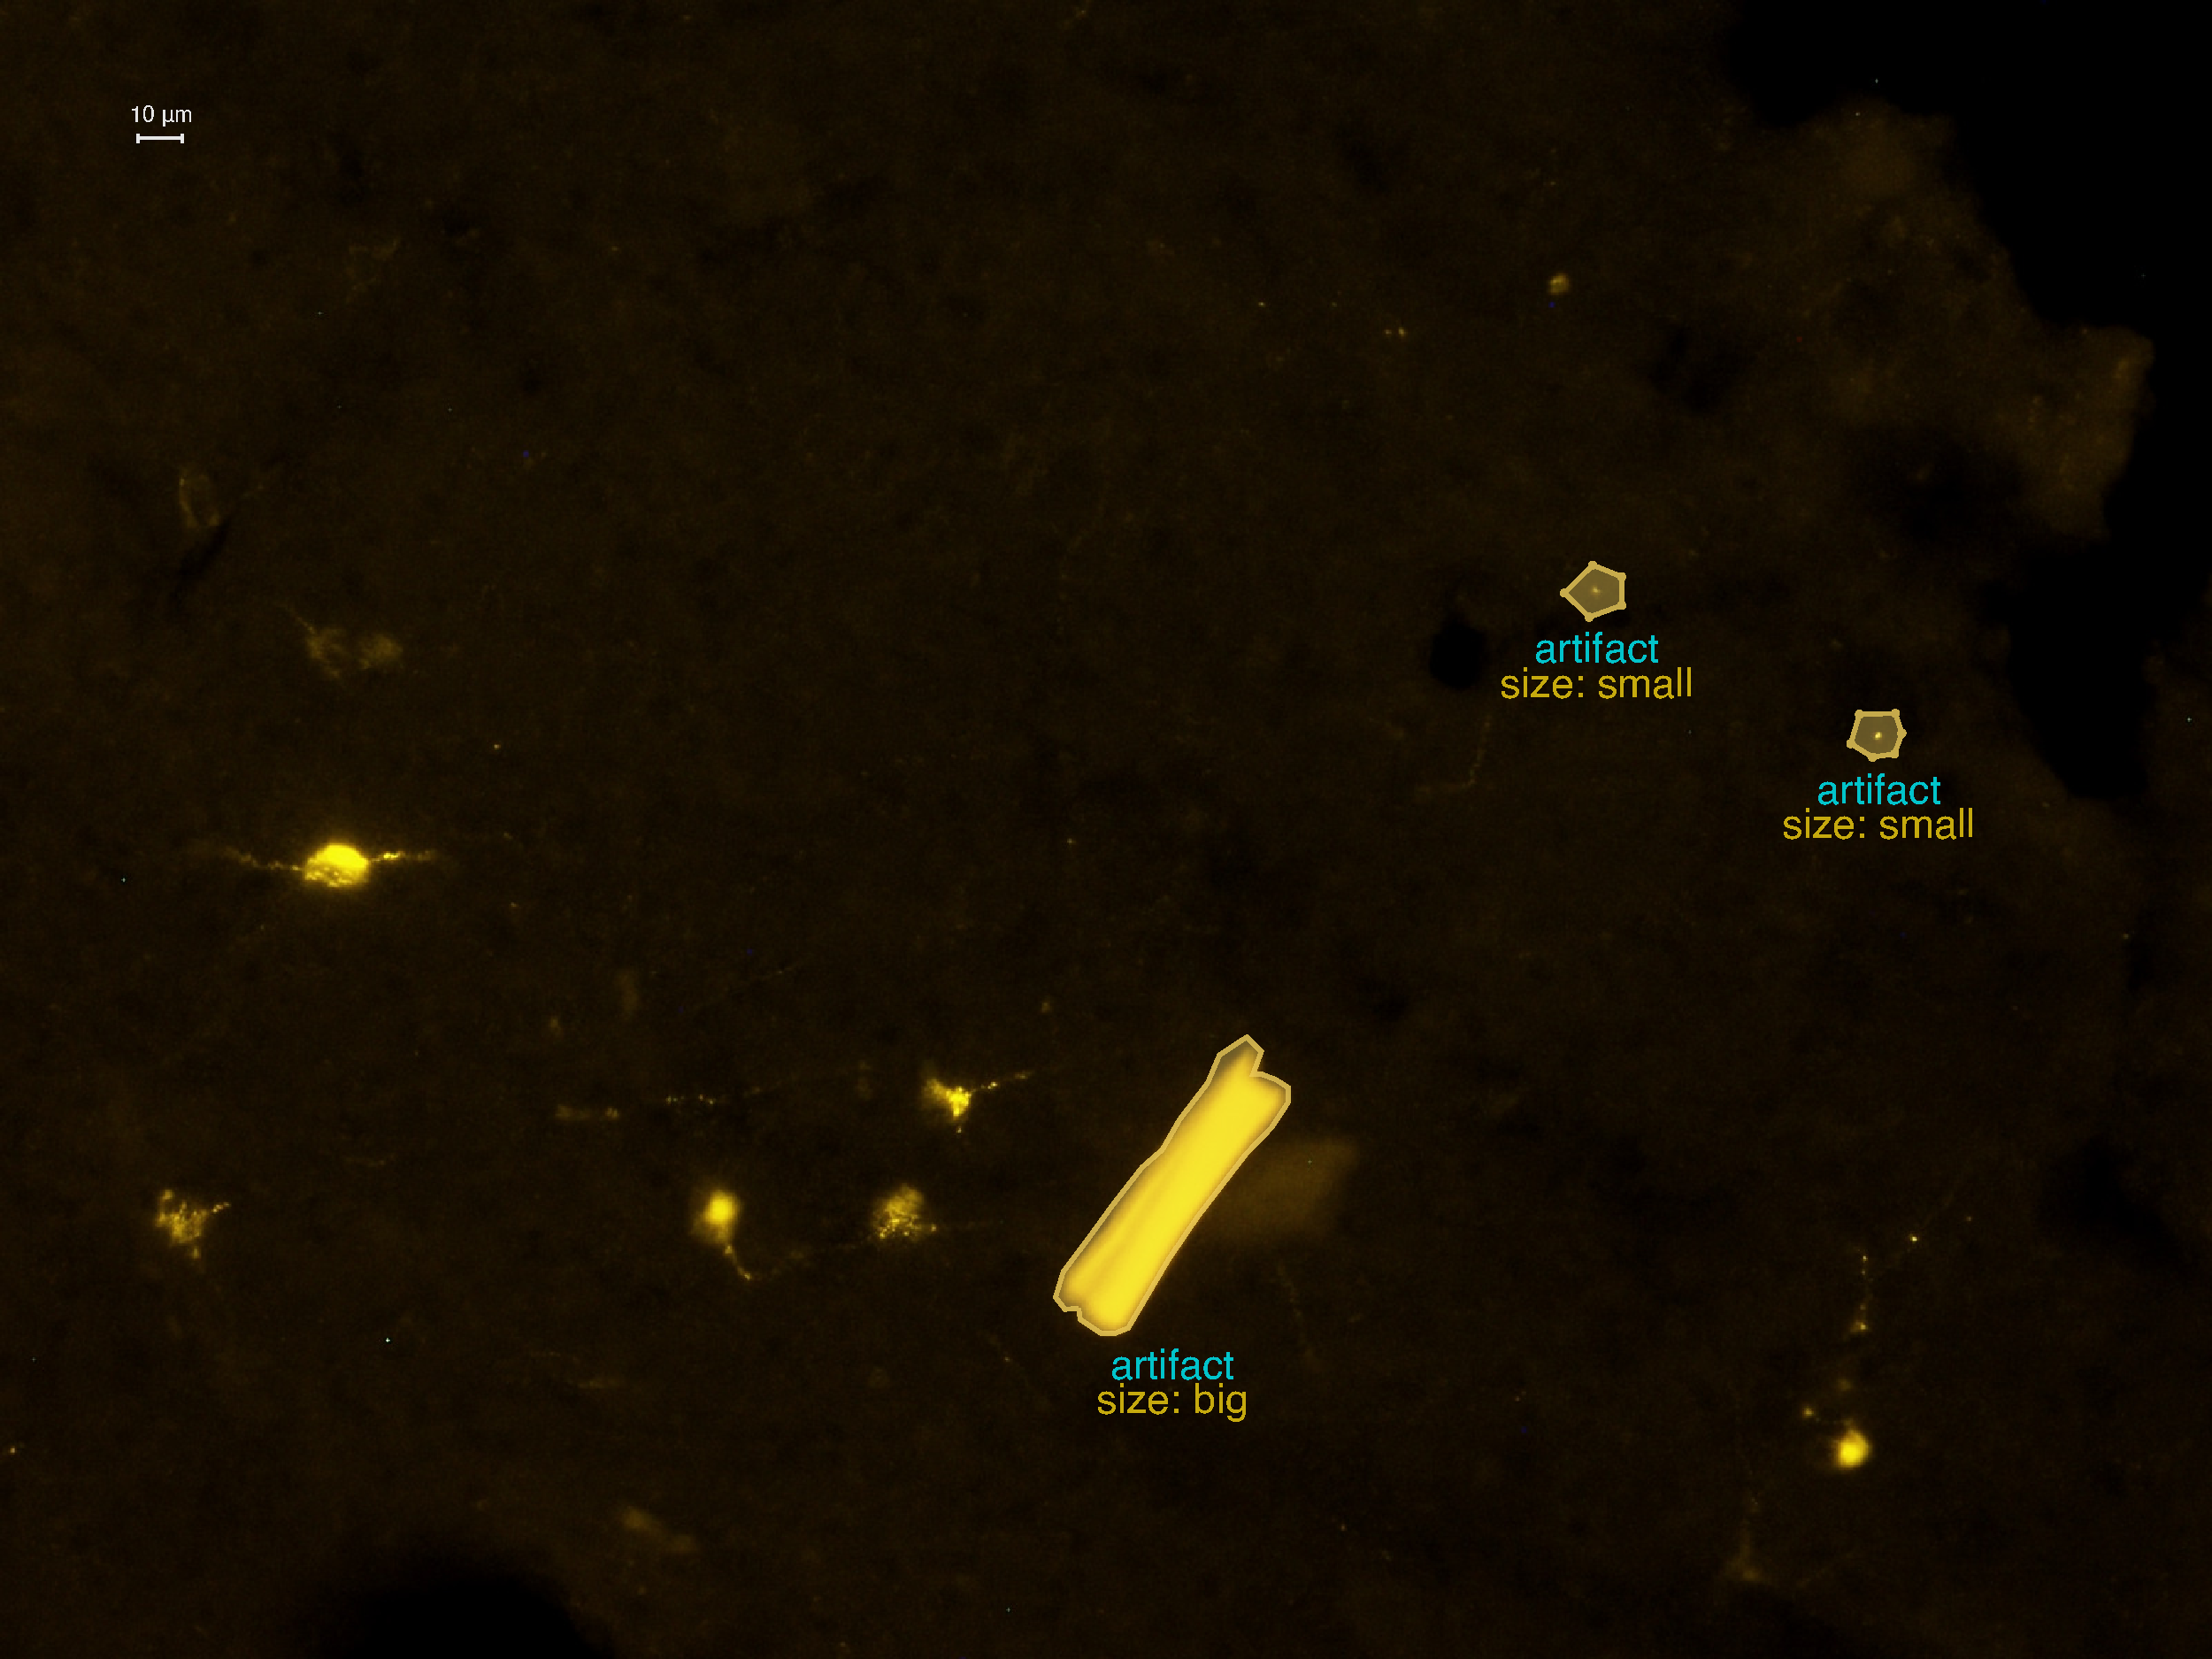
\includegraphics[width=\linewidth]{figures/120_dataset/challenges/artifacts.pdf}\label{fig:artifacts:macaroon}
    }
    \caption{\textbf{Challenges and artifacts. (3)}
    The fluorophore may accumulate in small (point-artifacts) or even large (``macaroni"-shaped artifact) areas; this causes emissions hard to distinguish from cells just looking at the pixels' color features.
    }
\end{figure}
\end{landscape}
\clearpage
\restoregeometry